\chapter{Security of the Diplomatiq application}
\label{chapter:security}

\section{Introduction}

\subsection{Motivation}

Web applications in general are notoriously insecure. According to an article by the prominent security firm Positive Technologies, statisticts of 2019 showed that hackers were able to hack users in 9 out of 10 web applications, exploiting vulnerabilities in the applications themselves~\cite{ptsecurity-2019}. The same article claims that breaches of sensitive data were a threat in 68\% of web applications, with the most breachable data being personal information and access credentials.

Having worked in cryptographic software development, I share the opinion that there is no such thing as too much software security. As on the one hand, Diplomatiq will store sensitive personal information from the beginning of its operation, and on the other hand, future diplomatic applications of the software will require strong security guarantees, I decided to put serious efforts to securing the Diplomatiq application. In this chapter, I present how I designed and implemented an application security framework addressing authentication, authorization, and data protection, providing cryptographic assurances regarding access control and the confidentiality and integrity of sensitive data.

\subsection{Scope and approach}

The implemented application security measures address all application layers across the front end and the back end of Diplomatiq. The front end needs to provide secure local data storage in the browser, as well as a variety of other security measures so the user can not be tricked into surrendering their password or other sensitive data. On the back end, the whole application needs to be secured, from the API's authentication and authorization mechanisms to the encrypted database records.

For securing the front end and the back end, I started off from my professional experience of securing a web application, and I also consulted the Open Web Application Security Project's web application security testing guide~\cite{owasp-webtestguide}. I implemented zero-knowledge user authentication using a suitable protocol, and I built a signing and authentication mechanism for HTTPS requests based on a symmetric cryptographic key hierarhcy, created upon the resulting shared key of the user authentication protocol. For authorizing sensitive API operations, I introduce the concept of session assurance level in order to make sure that the logged user is indeed themselves, and not an attacker who hijacked a user's session.

\section{Implemented cryptographic structures}

\subsection{DiplomatiqAEAD}

DiplomatiqAEAD is an \emph{Authenticated Encryption with Associated Data} structure, providing binary serialization and deserialiaztion capabilities. It essentially consists of an encrypted secret value and a public value attached to it, while the whole structure is authenticated, meaning it can not be modified without detection.

For the authenticated encryption, I chose today's prevalent Advanced Encryption Standard (AES) algorithm with 256-byte-long keys, in the more and more popular Galois/Counter Mode (GCM). AES-GCM provides strong confidentiality and ensures integrity of both the ciphertext and the additional authenticated data.

Although it does not contain self-implemented low-level cryptographic elements, DiplomatiqAEAD can be regarded as a cryptographic primitive within Diplomatiq applications, since it is a basic cryptographic building block of the system's authentication and database encryption infrastructure. The structure is used for transmitting encrypted and authenticated data across the front end and the back end application. This requires that the structure can be serialized in a self-contained way — meaning it must contain all necessary metadata needed for decryption as well —, and also that the two implementations on two different platforms are compatible with each other.

Similarly to other block cipher modes of operation, GCM also needs an initialization vector for a properly randomized output. According to the recommendation of the National Institute of Standards and Technology — a prevalent actor in cryptographic standards as well —, the initialization vector should be unique and 12 bytes long for efficient calculations~\cite{dworkin2007sp}. The initialization vector is also needed for decryption, so it needs to be included in the serialized packet. The output of AES-GCM is the ciphertext and an authentication tag, which is essentially a digest of the ciphertext, the initialization vector, and the additional authenticated data, verifying the integrity of all three. Most cryptography APIs append the authentication tag to the end of the ciphertext. As the authentication tag is needed for performing decryption, it needs to be included in the serialized packet.

For encoding the initialization vector, the ciphertext, the additional authenticated data and the authentication tag as a binary structure, I created a lightweight binary serialization scheme for DiplomatiqAEAD.\footnote{Although there are established standards like ASN.1, I decided that using it for this simple purpose only would cause more pain than gain.} The scheme consists of a header and a body. The body consists of the initialization vector, the additional authentication data, the ciphertext, and the authentication tag, in this order. Since each part of the body can essentially be of arbitrary length, the header contains each body part's length encoded on a fixed length: the length of the initialization vector on 1 byte, the length of the ciphertext on 4 bytes, the length of the additional authenticated data on 4 bytes, and the length of the authentication tag on 1 byte. All lengths are encoded in big-endian byte order, in unsigned magnitude representation. Encoding the length of the ciphertext and the additional authenticated data on 4 bytes introduces a planned constraint that DiplomatiqAEAD can be used only for encrypting and authenticating maximum 4 gigabytes of data at once. \Cref{fig:aead} presents the binary serialization format of DiplomatiqAEAD.

\begin{figure}[!htb]
    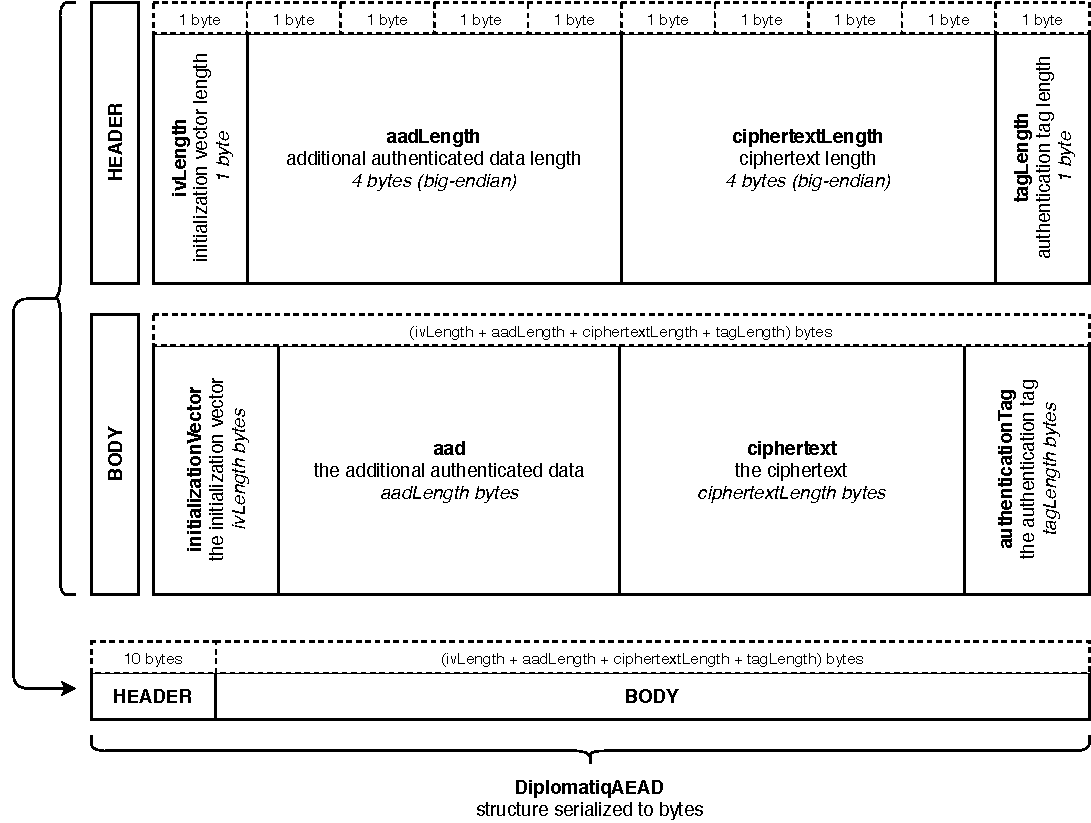
\includegraphics[width=\textwidth]{figures/aead.pdf}
    \caption{The structure of DiplomatiqAEAD serialized to bytes}
    \label{fig:aead}
\end{figure}

\section{Applied web platform security measures}

\subsection{Cross-Site Scripting (XSS)}

Cross-Site Scripting (XSS) attacks are a type of code injection, in which malicious scripts are injected into otherwise benign and trusted websites. XSS attacks occur when an attacker uses a web application to send malicious code, generally in the form of a browser side script, to an end user. Flaws that allow these attacks to succeed are quite widespread and occur anywhere a web application uses input from a user within the output it generates without validating or encoding it~\cite{owasp-xss}. Although in most modern browsers, a strong Content Security Policy ruleset disabling inline JavaScript can mitigate XSS, in older browsers the \lstinline{X-XSS-Protection} header can be used to instruct the browser to prevent rendering the page if an XSS attack is detected. Diplomatiq includes the \lstinline{X-XSS-Protection} header into its responses. The Angular framework also implements strong XSS mitigation measures: as long as their built-in filtering is used to display dynamic data in the browser, the application is protected. Diplomatiq uses Angular's built-in filtering.

\subsection{Content Security Policy (CSP)}

The Content Security Policy browser mechanism allows websites and web applications to specify what kind of resourcs (e.g. images, stylesheet files, script files, font files) can be loaded within the context of the application, and what kind of domains can the application connect to via network calls. This can protect against XSS attacks, and can also protect against performing unauthorized API calls. Diplomatiq applies a very strict Content Security Policy ruleset, which restricts everything by default, and only allows loading images, script files, stylesheet files, and font files from the application's very own domain name. Inline scripts are not allowed, meaning the application is safe against XSS attacks. Diplomatiq's policy allows connecting the front end application to \emph{api.diplomatiq.org} only.

\subsection{Cross-Origin Resource Sharing (CORS)}

By default, web browsers enforce the same-origin policy, meaning a web application running on a given domain can not initiate network requests to another domain. The Cross-Origin Resource Sharing mechanism instructs the browser to allow an application running on a certain origin to connect to a domain different than its origin. CORS settings are communicated to browsers via additional HTTP headers, specifying the origins which are allowed to connect to the domain which issued the headers. The Diplomatiq back end application issues CORS headers, which authorizes the application running under \emph{app.diplomatiq.org} to connect to the back end. No other application is authorized other than Diplomatiq's front end application.

\subsection{Feature Policy}

The Feature Policy experimental mecahnism enables to deny the usage of browser features for a web application, such as the browser's geolocation API, camera API, vibrate API, full screen API, etc. Feature Policy settings are communicated to the browser via a \lstinline{Feature-Policy} header. Their Feature Policies being the strictest, Diplomatiq's applications are not authorized to use such browser APIs at all.

\subsection{Referrer Policy}

The Referrer Policy mechanism can mitigate threats associated with the \lstinline{Referer}\footnote{The \lstinline{Referer} header is a misspelling of word \textquote{referrer}.} header. The \lstinline{Referer} header contains the URL of the page which the user visited before navigated to the current page. Referrer Policy settings are communicated to the browser via the \lstinline{Referrer-Policy} header. Their Referrer Policies being the strictest, Diplomatiq's applications omit the \lstinline{Referer} header entirely.

\subsection{Preventing click-jacking}

Click-jacking is a type of attacks where a page is embedded into another page via an \lstinline{<frame>} or \lstinline{<iframe>} element, and the user's clicks are hijacked to perform additional interactions on other web sites. Click-jacking can be prevented by instructing browsers not to allow embedding an application. Although Diplomatiq's restrictive Content Security Policy protects against this in modern browsers, in older browsers the \lstinline{X-Frame-Options} header should be set to \lstinline{DENY}. Diplomatiq's applications set this header accordingly as well.

\section{Authentication and authorization}

\subsection{Introduction, motivation, and terminology}

Broken and insecure authentication schemes are a constant problem of web applications~\cite{ptsecurity-2019}. On the list summarizing the top then security vulnerabilities of the Open Web Application Security Project, broken authetication is located in the second place~\cite{owasp-topten}.

Besides an authentication scheme being technically correct — it uses suitable protocols and hides sensitive information by techniques like encryption —, it also needs to provide additional guarantees on ensuring a user's identity. Password-only authentication is a contributing factor in most authentication attacks~\cite{ptsecurity-2019}. Times are changing: yesterday's recommendations on authentication systems based on strong, frequently changing passwords are replaced with more modern approaches based on multiple factors of authentication. NIST explicitly advises to organizations that instead of focusing on password policies, incorporate multi-factor authentication solutions into their systems~\cite{nistidguide}.

I wanted to get authentication and authorization right in Diplomatiq's systems. For certain sensitive interactions, I wanted to provide additional guarantees on the user's identity — beyond the standard approach that \textquote{authenticate the user \emph{only once} based on their password and an additional second factor, then later in any point in time believe without verification that the user sitting in front of the computer is still the same} — to avoid stealing session credentials. I also wanted to be able to further encrypt sensitive between the client and the server. Even though all communications are already done encrypted over Transport Layer Security, I still believe there is no such thing as too much security — as long as it does not mean a worse user experience.

In the following, I use the term authentication in two different contexts. \emph{User authentication} means that the user cryptographically proves to the server, that they are in posession of a valid password, which corresponds to the given email address, then performs a second step of email-based authentication. In essence, \emph{user authentication} means a user logs in to Diplomatiq. The process of user authentication results in a set of \emph{login credentials}, which the client stores locally, encrypted. \emph{Request authentication} means that the client cryptographically proves to the server that they are in posession of valid login credentials, without sending the actual credentials over the network. In essence, request authentication happens on a per-API-request basis, and essentially means that when the logged in user's Diplomatiq client application performs a request against Diplomatiq's API, the API checks if the client provided a legitimate cryptographic proof about the posession of the necessary credentials. The goal of user and request authentication is to get a strong proof about the user's identity.

In the following, the term authorization means that an already authenticated user is checked by the server whether they have the necessary level of access and level of \emph{session assurance} to perform a given API operation. Basically this is the same as the original meaning of authorization, but Diplomatiq's authorization scheme incorporates the elapsed \emph{time} into the authorization. A session's assurance level can be elevated with re-authenticating, meaning an elevated session assurance level provides a stronger proof about the user's identity sitting in front of the computer at a given point in time.\footnote{After the specified time, the assurance level expires, and a user needs to re-authenticate again for sensitive operations.} Similarly to request authentication, authorization also happens on a per-request basis, and the request is rejected if the user does not have the required level of access.

\subsection{Why not OpenID Connect or OAuth 2.0?}

There are several already established, mature authentication and authorization standards on the market, like OpenID Connect\footnote{https://openid.net/connect}~\cite{openid-connect-core} for authentication, and OAuth 2.0\footnote{https://oauth.net/2}~\cite{rfc6749} for authorization. Having implemented several applications upon both methodologies, I have some, but not exhaustive experience on using these standards. After further inspections, I concluded that neither solutions would satisfy all my below specified requirements.

Not implementing OAuth 2.0 introduces a restriction of federated authentication, meaning users will not be able to authenticate themselves to Diplomatiq with e.g. their social media accounts. This question does not get addressed in this thesis.

\subsection{Requirements}

In the following, I summarize the requirements I formulated regarding Diplomatiq's authentication and authorization framework, and I also describe the threats they mitigate.

\subsubsection{Zero-knowledge password proof}

User authentication should be implemented upon a \emph{zero-knowledge password proof} scheme. The client should be able to verify to the server, that the user knows the password, without the password or its any derivative form ever leaving the client or being transmitted over the network. The server should store neither the user's password, nor any password-equivalent data. This prevents attackers from stealing user passwords either over the network, or by breaking into the back end application's database.

\subsubsection{Mandatory multi-factor authentication}

Beyond password, a mandatory second factor of authentication should be used for user authentication. This prevents attackers to perform password-based authentication and impersonate the user.

\subsubsection{No personal data for request authentication}

No personally identifiable data should be used for authenticating a network request. This implies that network traffic between the client and the server should not contain personally identifiable information about the authenticated user by default, unless of course the request's actual payload contains such information to be stored on the server. This is a further layer of protection over Transport Layer Security.

\subsubsection{Shared symmetric key between the client and the server for encryption and signing}

User authentication should result in a long-term shared symmetric key between the client and the server for performing further encryption of very sensitive data and credentials transmitted over the network. This prevents attackers to obtain plaintext credentials if they somehow manage to steal and decrypt and encrypted network request over TLS.

\subsubsection{Signed network requests}

Authenticated network requests should be signed, and the signature should incorporate all characteristics of the request, including its timestamp. The request should be rejected by the server if the signature is invalid, or if the timestamp is outside a given interval to the current time. This prevents attackers to replay a network request if they somehow manage to steal one over TLS.

\subsubsection{Time-based session assurance levels}

The scheme should provide a way to ascertain the user identity before performing sensitive operations. That is, the scheme should incorporate assurance levels for sessions in the meaning of a higher assurance level means a higher certainty regarding the identity of the user sitting in front of the computer at a given point in time. Sensitive API operations should require a higher session assurance level. This prevents attackers to perform sensitive API operations impersonating the user, who left their computer unlocked.

\subsubsection{Immediate logout}

The scheme should not rely solely on expiring entities. Request credentials should be authenticated and authorized for every request, and this should always incorporate checking the validity of the provided credentials. This implies that access tokens should be stored on the server, along with their expiry. This prevents attackers from stealing abandoned access credentials, which have not yet expired.

\subsection{Protecting endpoints}

Diplomatiq endpoints can be split into two parts:

\begin{itemize}
\item \emph{Unauthenticated} (i.e. \textquote{not logged in}) endpoints are publicly available for every user, and they do not need to be able to identity the user. They do not require signed requests.
\item \emph{Authenticated} (i.e. \textquote{logged in}) endpoints are available after performing user authentication only. These endpoints require the user to be identifiable, and requests to be signed.
\end{itemize}

Endpoints are protected using filters implemented in Spring Boot. Filters are ordered, and executed sequentially. They can either forward, modify or even reject the request with an error. As described later, both authenticated and unauthenticated are protected by filters.

\subsection{User authentication}

\subsubsection{Proving the knowledge of the password without ever revealing the password}

For performing zero-knowledge password-based authentication, I decided to use the Secure Remote Password (SRP) protocol's latest, 6a version~\cite{rfc2945}. SRP is an augmented password-authenticated key agreement (PAKE) protocol, which specifies a set of cryptographic methods for performing password-based authentication between two parties over an insecure channel, without sending the password or its any derivative over the channel. Similarly to other PAKE protocols, an attacker obtaining the network traffic\footnote{Since Diplomatiq uses TLS, it is unlikely that an attacker would be able to eavesdrop client-server communication} of the authentication would not be able to perform an exhaustive search for the password, based solely on the obtained network data. Since the server does not store the password, even if an attacker steals the server's database, they would not be able to impersonate the user, unless they perform an exhaustive key search for the password first, based on the stolen data.

The authentication results in a shared, symmetric session key between the parties. The protocol provides strong cryptographic proof to both parties that they successfully authenticated against each other, i.e. the server can cryptographically verify the password.

\subsubsection{Logging in}

The user authentication flow consists of the following steps:

\begin{enumerate}
\item The client initiates SRP's password authentication process by providing their email address to the server, and receives a response with the server's cryptographic challenge value.
\item The client performs cryptographic calculations on the challenge value, mixing the password's one-way hash\footnote{For hashing, Diplomatiq uses the \emph{scrypt} password-based key derivation function to slow down attackers, who want to perform an exhaustive search for the password~\cite{rfc7914}.} into the calculations, eventually resulting in a value called a \emph{password proof}. The password proof does not have a direct relation to the plaintext password itself, but it is based on the server challenge value and the password, and allows the server to verify that the client is indeed in posession of the valid password. With this step, the client has completed the password authentication, and the client and the server has a shared cryptographic key, which I named \emph{authentication session key}, and the client is in possession of an authentication session.
\item To perform the login operation, which results in a \emph{client device} authorized to acquire a \emph{session}, the user needs to complete multi-factor authentication. This involves receiving an email with a code expring in 5 minutes, and providing the code to the server. Performing multi-factor authentication elevates the user's authentication session from password-elevated level to multi-factor elevated level.
\item With a multi-factor elevated authentication session, the user is authorized to call the login operation. This issues a \emph{client device} with a device identifier, and returns a \emph{device key} and a long-term \emph{session token}. The device identifier, device key and session token are both encrypted values, wrapped into a DiplomatiqAEAD structure. The device key is encrypted with the authentication session key, and the device identifier and the session token is encrypted with the device key. To acquire the device identifier and the session token, the client first decrypts the device key with the authentication session key, then decrypts the device identifier and the session token. The device identifier is required to identify, which device of which user calls the API, and the session token is a long-term secret credential authorizing the issued device to acquire a session after completing the login flow.
\item With a logged-in device, the client device is authorized to acquire a session, by providing a session token to the server. The session token is a sensitive credential, therefore it is sent encrypted with the device key.
\item After acquiring a session, the client can perform calls against the API, providing valid request authentication with the session credentials.
\end{enumerate}

\Cref{fig:login} dispalys a summary of the above user authentication scheme. The main security characteristics of the scheme is provided by the cryptographic key hierarchy built upon the authentication session key, which was actually never transmitted over the network. Instead, it was calculated independently on the server and on the client, as a result of the authentication procedure described by the SRP protocol. Essentially all further credentials and cryptographic keys are (transitively) encrypted with this authentication session key, which is impossible to be eavesdropped by an attacker, as it does not leave machines.

\begin{figure}[!htb]
    \centering
    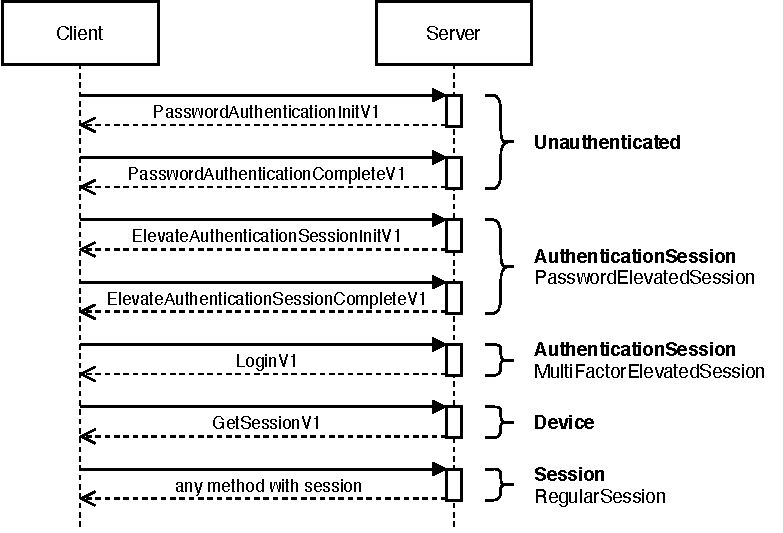
\includegraphics[width=\textwidth-1cm]{figures/login.pdf}
    \caption{The login flow}
    \label{fig:login}
\end{figure}

\subsubsection{Securely storing login session credentials locally}

After performing the user authentication, the client needs to persist the credentials of the issued device locally in a secure way. For this, I introduce a device container, which is an encrypted container for storing sensitive credentials in the client browser's local storage. The device container is essentially a DiplomatiqAEAD structue, encrypted with the \emph{device container key}. The device container is never persisted in unencrypted form.

For automatically logging in the user in a given web browser by data stored in a device container as a result of a previous login, the device container key needs to be queried from the server on a public endpoint.\footnote{At this point, the client does not access its credentials, as they are in the encrypted device container.} This key can be regarded as a not-so-sensitive data, since even if an attacker obtains a device container key, they would still need the actual device container, which is stored only in the browser's local storage.

\subsection{Request authentication}

\subsubsection{Overview}

After the user has authenticated themselves by logging in into Diplomatiq, each API request initiated by the user is also authenticated and authorized one-by-one. In this section I present different authentication schemes authenticating with different credentials over the user's authentication lifecycle, and I introduce the concept of session assurance levels.

\subsubsection{Authentication schemes}

From the point of a user entering their password to the first successful \textquote{logged-in} API call, there are several steps. These steps were introduced previously, and now I present the underlying authentication schemes I implemented. Schemes are essentially the definitions of how the request should be authenticated, and how the request's signature needs to be checked. All schemes are versioned in order to be changed on demand.

The \emph{Unauthenticated} \textquote{authentication scheme} does not require the user to be authenticated, as its name suggests. It does not require signed requests, but it requires that the client includes the client identifier header, and also requires the client clock will be in sync with the server's clock. The client identifier and the clock synchronization is detailed later.

The \emph{AuthenticationSessionSignatureV1} scheme is used during the password and multi-factor authentication flow of the login process. The authentication session is identified by the authentication session id, and the request is signed with the authentication session key the client and the server mutually agreed on.

The \emph{DeviceSignatureV1} scheme is used after the user performed the password and multi-factor authentication, and logged in, meaning performed a call to the login endpoint, which issued a client device to them. As previously mentioned, this long-term device has a device key, and a session token issued to them. Requests performed with the this scheme is signed with the device key, and identified by the attached device id as a header. Actually, this scheme is used for only two purposes: getting a session with the session token and logging out.

The \emph{SessionSignatureV1} scheme is used after the user acquired a session. This scheme is used for every regular API call, and its requests are signed with the device key, and identified by the device key and the session key attached as headers.

\Cref{fig:authentication-schemes} displays a detailed summary about authentication session schemes.

\begin{figure}[!htb]
    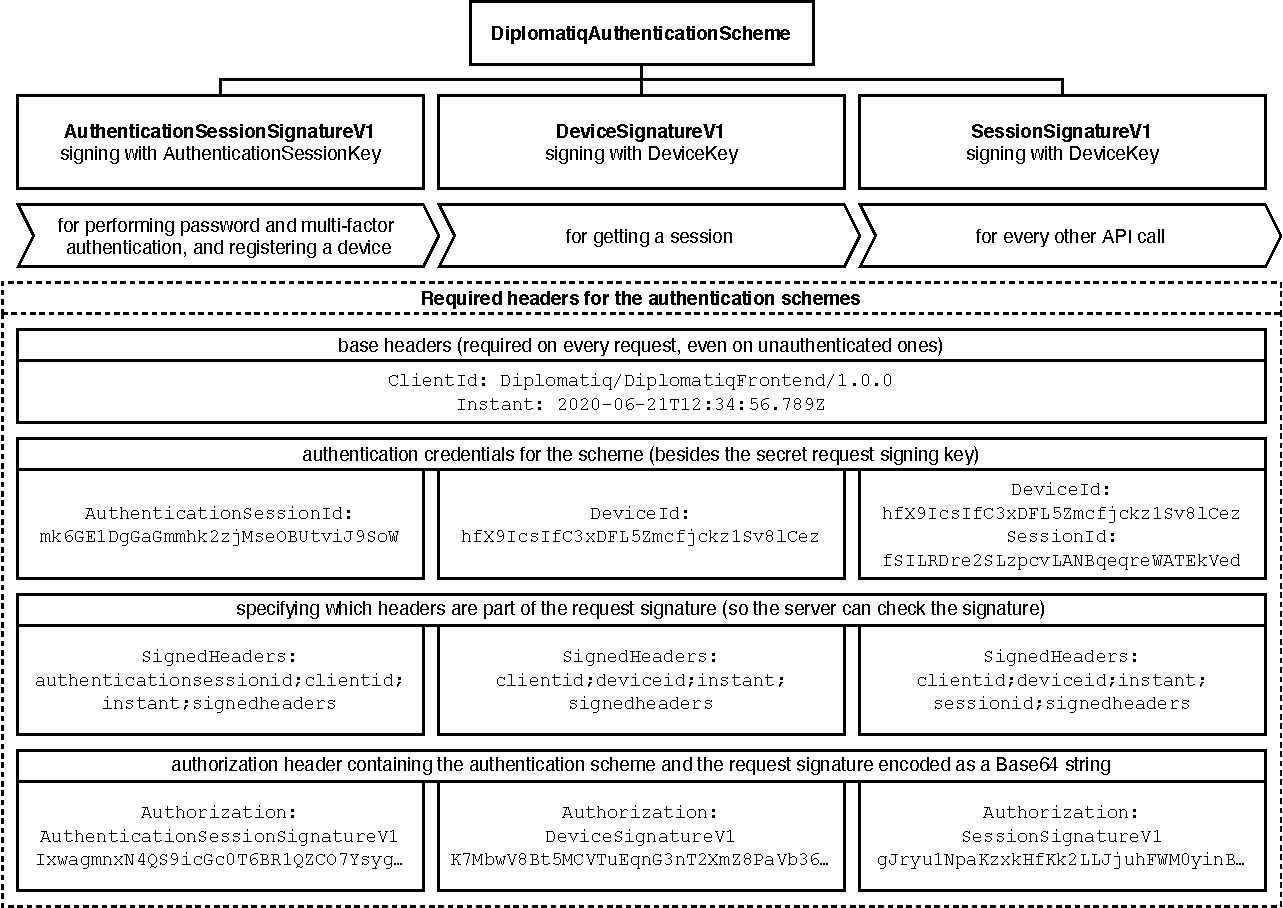
\includegraphics[width=\textwidth]{figures/authentication-schemes.pdf}
    \caption{A summary of Diplomatiq's authentication schemes}
    \label{fig:authentication-schemes}
\end{figure}

\subsubsection{Session assurance levels}

There are certain very sensitive API methods and operations, which can require to re-authenticate the user. Such methods implemented in Diplomatiq are password change or cancelling a conference application, which require the user's current password. More sensitive methods, such as cancelling a whole conference or deleting a user account require both the user's password and performing multi-factor authentication. These safeguards are implemented to make sure that the user really is who she says she is, and not an attacker with malicious intents. For handling these kinds of safeguards in a uniform way instead of ad-hoc re-authentication solutions, I introduce the concept of \emph{session assurance levels}. A higher session assurance level provides a higher assurance about the current user's identity, as a result of a higher level of re-authentication.

In the extensible, hierarchical system I defined the following assurance levels:

\begin{itemize}
\item \emph{RegularSession} is the lowest assurance level. It assures that a user is logged in, and can be renewed without user interaction following its 1-hour expiry.
\item \emph{PasswordElevatedSession} is the medium assurance level. It is valid for 15 minutes from point the user provided a valid password, thus it essentially proves that the user provided correct password in the last 15 minutes.
\item \emph{MultiFactorElevatedSession} is the highest assurance level. It is valid for 5 minutes from the point the user completed a multi-factor authentication flow. \emph{MultiFactorElevatedSession} assurance level can only be acquired with a \emph{PasswordElevatedSession} assurance level. This assurance level therefore proves that in the last 15 minutes, the user provided correct password, and in the last 5 minutes, they completed a multi-factor authentication flow through their email address, and Diplomatiq can be pretty sure that the user is who she says she is.
\end{itemize}

\Cref{fig:session-assurance-levels} displays a summary of the above assurance levels. Sequence diagrams presenting the process of a session elevation can be found in the Appendix.

\begin{figure}[!htb]
    \centering
    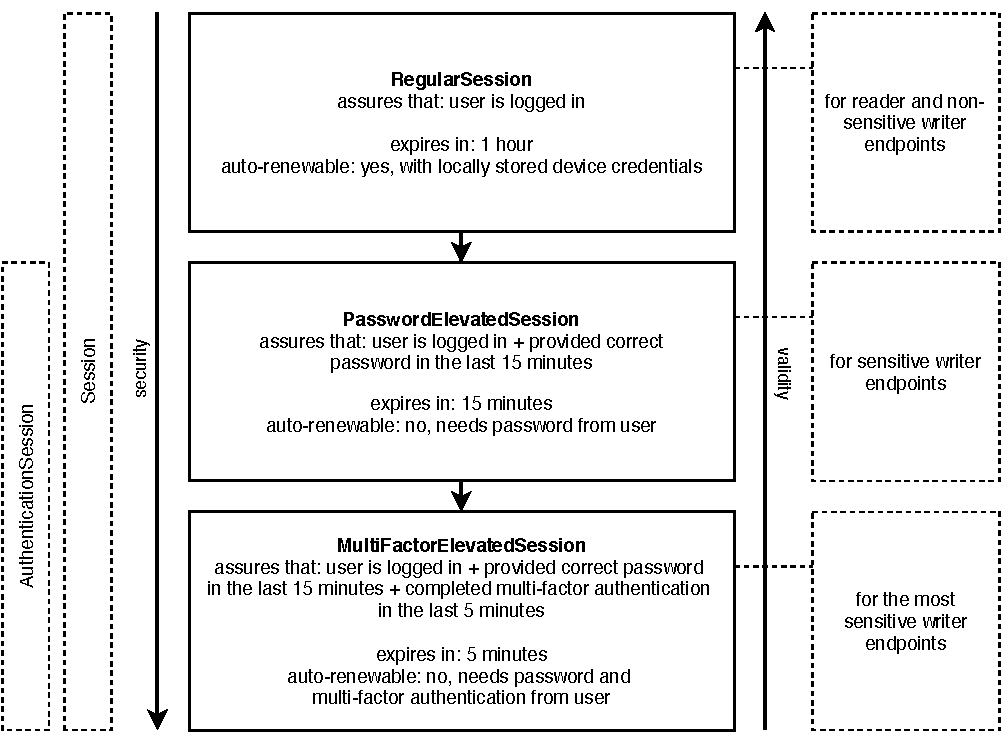
\includegraphics[width=\textwidth-1.5cm]{figures/session-assurance-levels.pdf}
    \caption{Diplomatiq's session assurance levels}
    \label{fig:session-assurance-levels}
\end{figure}

An authentication session level is bound to a set of API methods implemented in separate controllers via Spring's controller proxy authorization. This means that if I want to create a method with a password-level session assurance, I just need to insert the method's definition in the controller defining password-level methods. As I already implemented the underlying infrastructure, there is no further configuration needed.

The session assurance levels are stored and handled on the server. The client does not even know about its credentials' current assurance level, it just tries to call the API with its current credentials, and retries after requesting password or multi-factor authentication whenever the server throws a \lstinline{SessionElevationRequired} error. Whenever a request arrives to the server, it checks if the targeted controller's required assurance level is met by the provided authentication credentials, and throws the previously mentioned error, if not.

\subsection{Client version identifier}

For logging purposes, every request against Diplomatiq's API must contain a \lstinline{ClientId} header, defining which Diplomatiq client's which version initiated the request to the API. In the future, when Diplomatiq has clients for desktop computers and smartphones, this header will also identify the platform. The current value of the \lstinline{ClientId} header is \emph{Diplomatiq/DiplomatiqFrontend/X.Y.Z}, where X, Y and Z are the client's version numbers according to the semantic versioning scheme. Requests lacking the \lstinline{ClientId} header are rejected.

\subsection{Client clock discrepancy}

It is unfortunate if the client's clock differs from the server's clock, because the client can display invalid data. Differing clocks can also break along the safeguards against replay attacks, since a client signing a request with wrong clock setting will not be able to create a valid signature. Therefore, every request against Diplomatiq's API must contain an \lstinline{Instant} header, which contains the client's current instant\footnote{Instant is a universal, instantaneous point on the time-line in the UTC time zone.} in the ISO~8601~\cite{iso8601} simplified string format, including date and time.\footnote{Such as: \lstinline{2020-05-31T23:59:59Z}}

\subsection{Signing requests}

In order to make cryptographically sure that requests originate from an authorized client, all authenticated requests against Diplomatiq's API must be signed with a key, which is determined by the endpoint's required authentication scheme. This allows the server to retrieve the client's signing key (such as a device key) by the attached request metadata (such as a device id provided in a request header), then verify that the attached signature was indeed created with the key.

On the one hand, this solution provides an additional layer of protection against request tampering on top of TLS, and on the other hand, since the request should contain its timestamp in the \lstinline{Instant} header, it also prevents attackers to perform replay attacks after somehow obtaining a plaintext request.

\begin{figure}[!htb]
    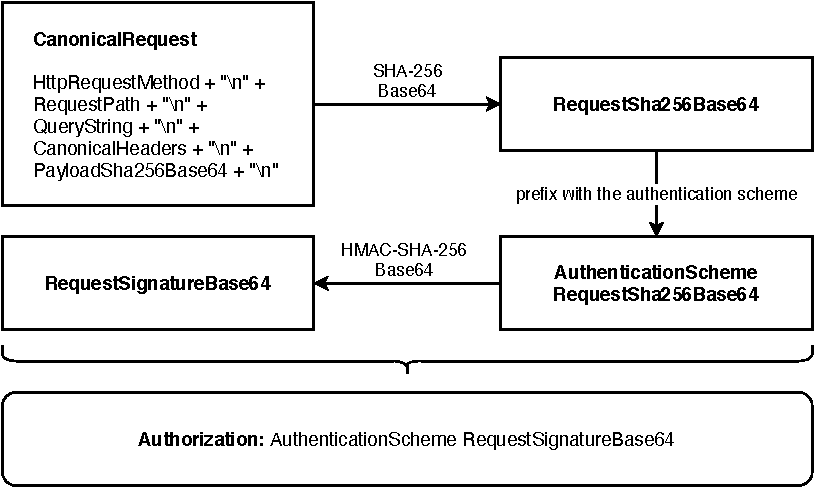
\includegraphics[width=\textwidth]{figures/request-signature.pdf}
    \caption{The process of signing a request}
    \label{fig:request-signature}
\end{figure}

\subsection{Implementing request authentication with Spring filters}

nem használunk spring sessiont

\begin{figure}[!htb]
    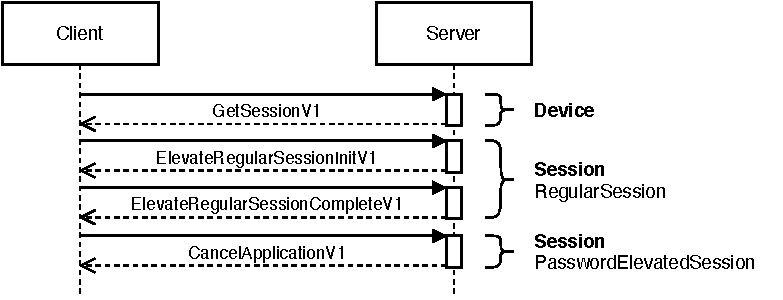
\includegraphics[width=\textwidth]{figures/elevate-to-password-session.pdf}
    \caption{Server calls for elevating a session to password level}
    \label{fig:elevate-to-password-session}
\end{figure}

\begin{figure}[!htb]
    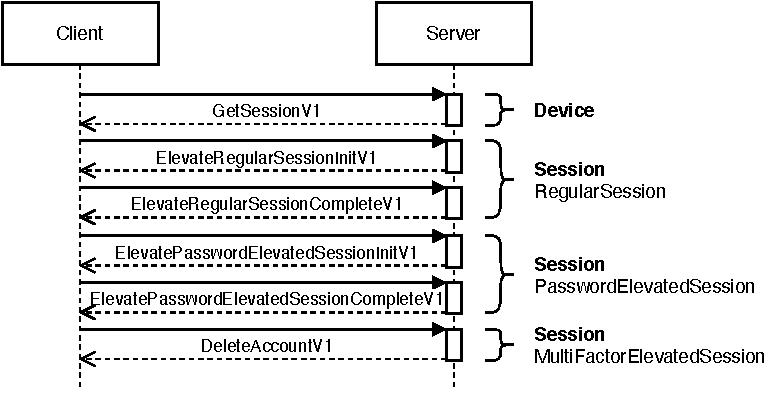
\includegraphics[width=\textwidth]{figures/elevate-to-mfa-session.pdf}
    \caption{Server calls for elevating a session to multi-factor level}
    \label{fig:elevate-to-mfa-session}
\end{figure}

\begin{figure}[!htb]
    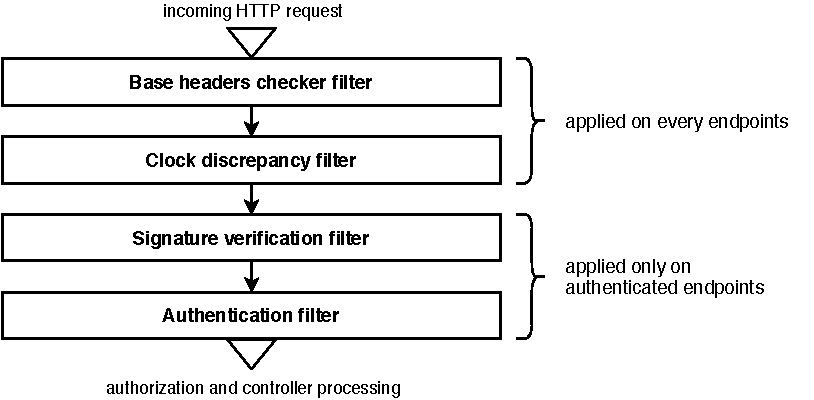
\includegraphics[width=\textwidth]{figures/request-filters.pdf}
    \caption{A summary of the back end application's request filters}
    \label{fig:request-filters}
\end{figure}

\begin{figure}[!htb]
    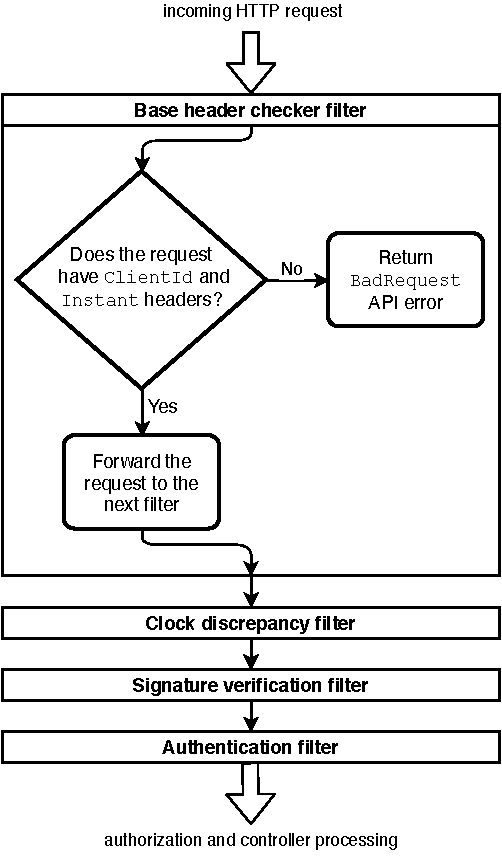
\includegraphics[width=\textwidth]{figures/base-headers-checker-filter.pdf}
    \caption{The base headers checker filter}
    \label{fig:base-headers-checker-filter}
\end{figure}

\begin{figure}[!htb]
    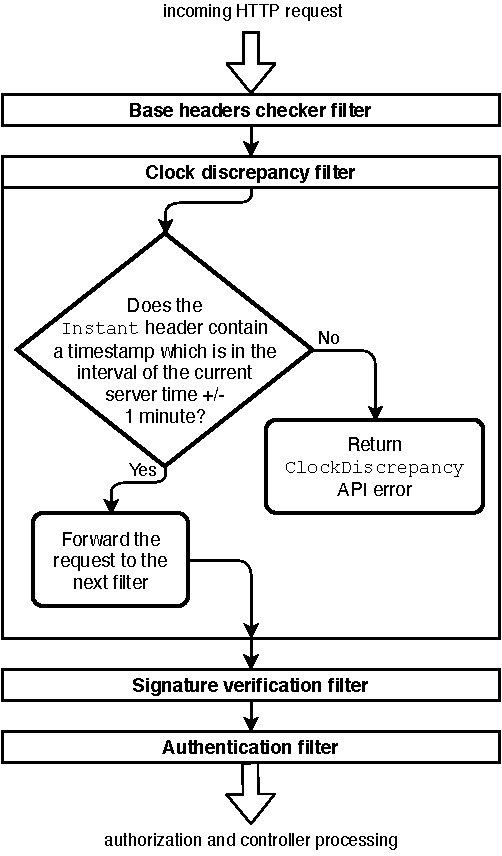
\includegraphics[width=\textwidth]{figures/clock-discrepancy-filter.pdf}
    \caption{The clock discrepancy filter}
    \label{fig:clock-discrepancy-filter}
\end{figure}

\begin{figure}[!htb]
    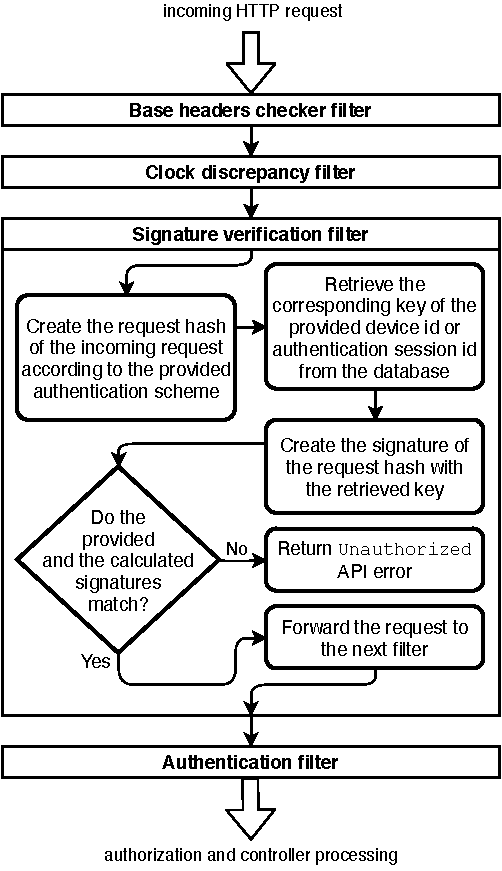
\includegraphics[width=\textwidth]{figures/signature-verification-filter.pdf}
    \caption{The signature verification filter}
    \label{fig:signature-verification-filter}
\end{figure}

\begin{figure}[!htb]
    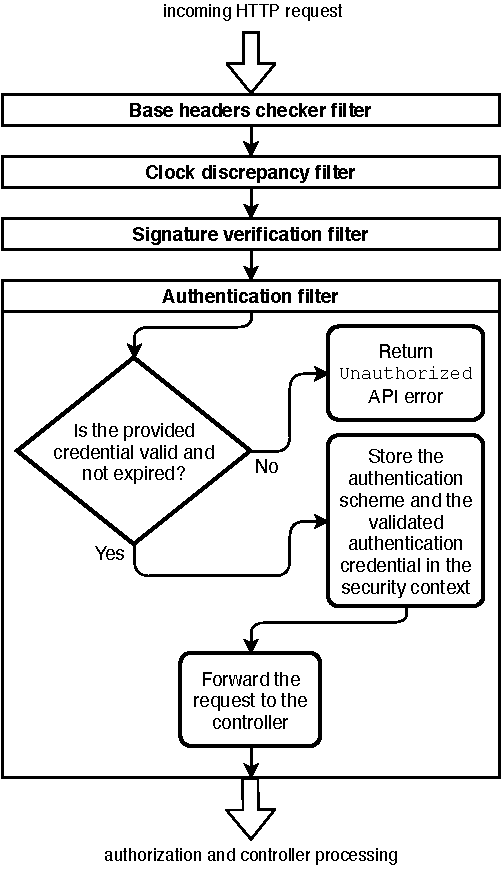
\includegraphics[width=\textwidth]{figures/authentication-filter.pdf}
    \caption{The authentication filter}
    \label{fig:authentication-filter}
\end{figure}

\begin{figure}[!htb]
    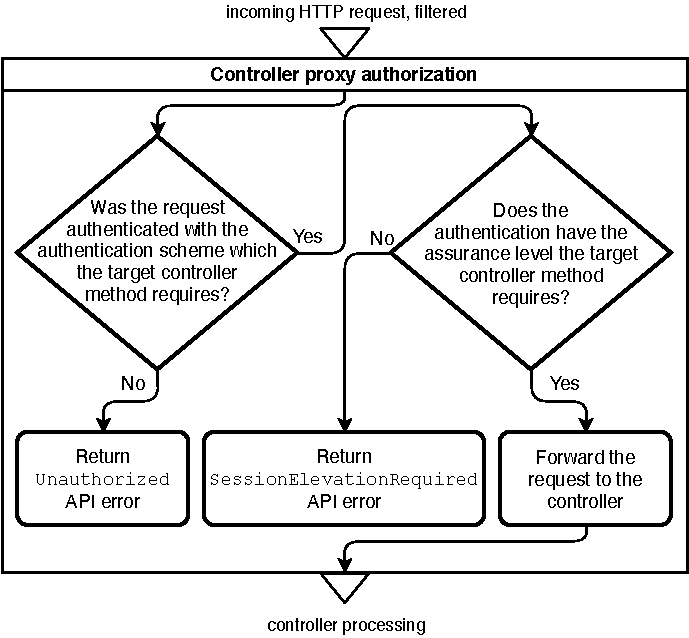
\includegraphics[width=\textwidth]{figures/controller-authorization.pdf}
    \caption{A summary of controller authorization}
    \label{fig:controller-authorization}
\end{figure}

\section{Encrypting sensitive data in the database}

encrypted db values, key versioning to avoid birthday problem

nem okozott mérhető változást a request

\section{Other security measures}

nem adunk ki a userről adatot (hogy létezik-e ilyen mailcímű user, stb)

device container key is queried no error

security.txt
